%*****************************************************************************************
%*********************************** Third Chapter **************************************
%*****************************************************************************************

\chapter{Proposed Framework and Timeline}

% **************************** Define Graphics Path **************************
\ifpdf
    \graphicspath{{Chapter3/Figs/Raster/}{Chapter3/Figs/PDF/}{Chapter3/Figs/}}
\else
    \graphicspath{{Chapter3/Figs/Vector/}{Chapter3/Figs/}}
\fi

% An illustration of the PhD work is shown in Figure \ref{fig:proposedapproach}.
The proposed framework is divided into five modules (Figure \ref{fig:proposedapproach}): 
1) Data acquistion using a Bluetooth body sensor network with Inertial Measurement Units, 
2) Reconstruction of the state space with a C++ class, 
3) nonlinear measuraments and feature extractions by means of Principal Component
Analysis, 
4) classification using state-of-the-art multiatribute machine learning algorithms, 
and  5) application(s) such as dacing, cycling. 
% Sensor data acquistion shall allow to acquire raw data from either 
% accelerometer, gyroscope or the use of euler angles. 
% Magnetometer-sensor based system would also provide important information regarding 
% the human motion activity. 
% The sensor's time series will be used to reconstruct the state space 
% by means of the taken's theorem.
% % two different operations will be performed:
% % evaluation of the methods to determine the $m$ and $\tau$ and 
% % implementation of the algororithms to compute $m$ and $\tau$. 
% % As was stated in Section 2, additional methods will be evaluated to compute
% % the reconstructed state space.
% Nonlinear measuraments such as Lyapunov Exponents, Poincar\'e maps, H\'enon maps,
% will then be investigated to characterize motion patterns. 
% One can hypothesize that by studying non-published concepts from nonlinear dynamics 
% for human activity recognition, different features can be used to 
% indentify human motion activities.
% Classification stage will include reviewing machine learning methods
% so as to choose an appropriate approach for the task at hand.
% Once human body activities can be recognized, we can use our approach in 
% different applications.

\begin{figure}[htbp!] 
\centering    
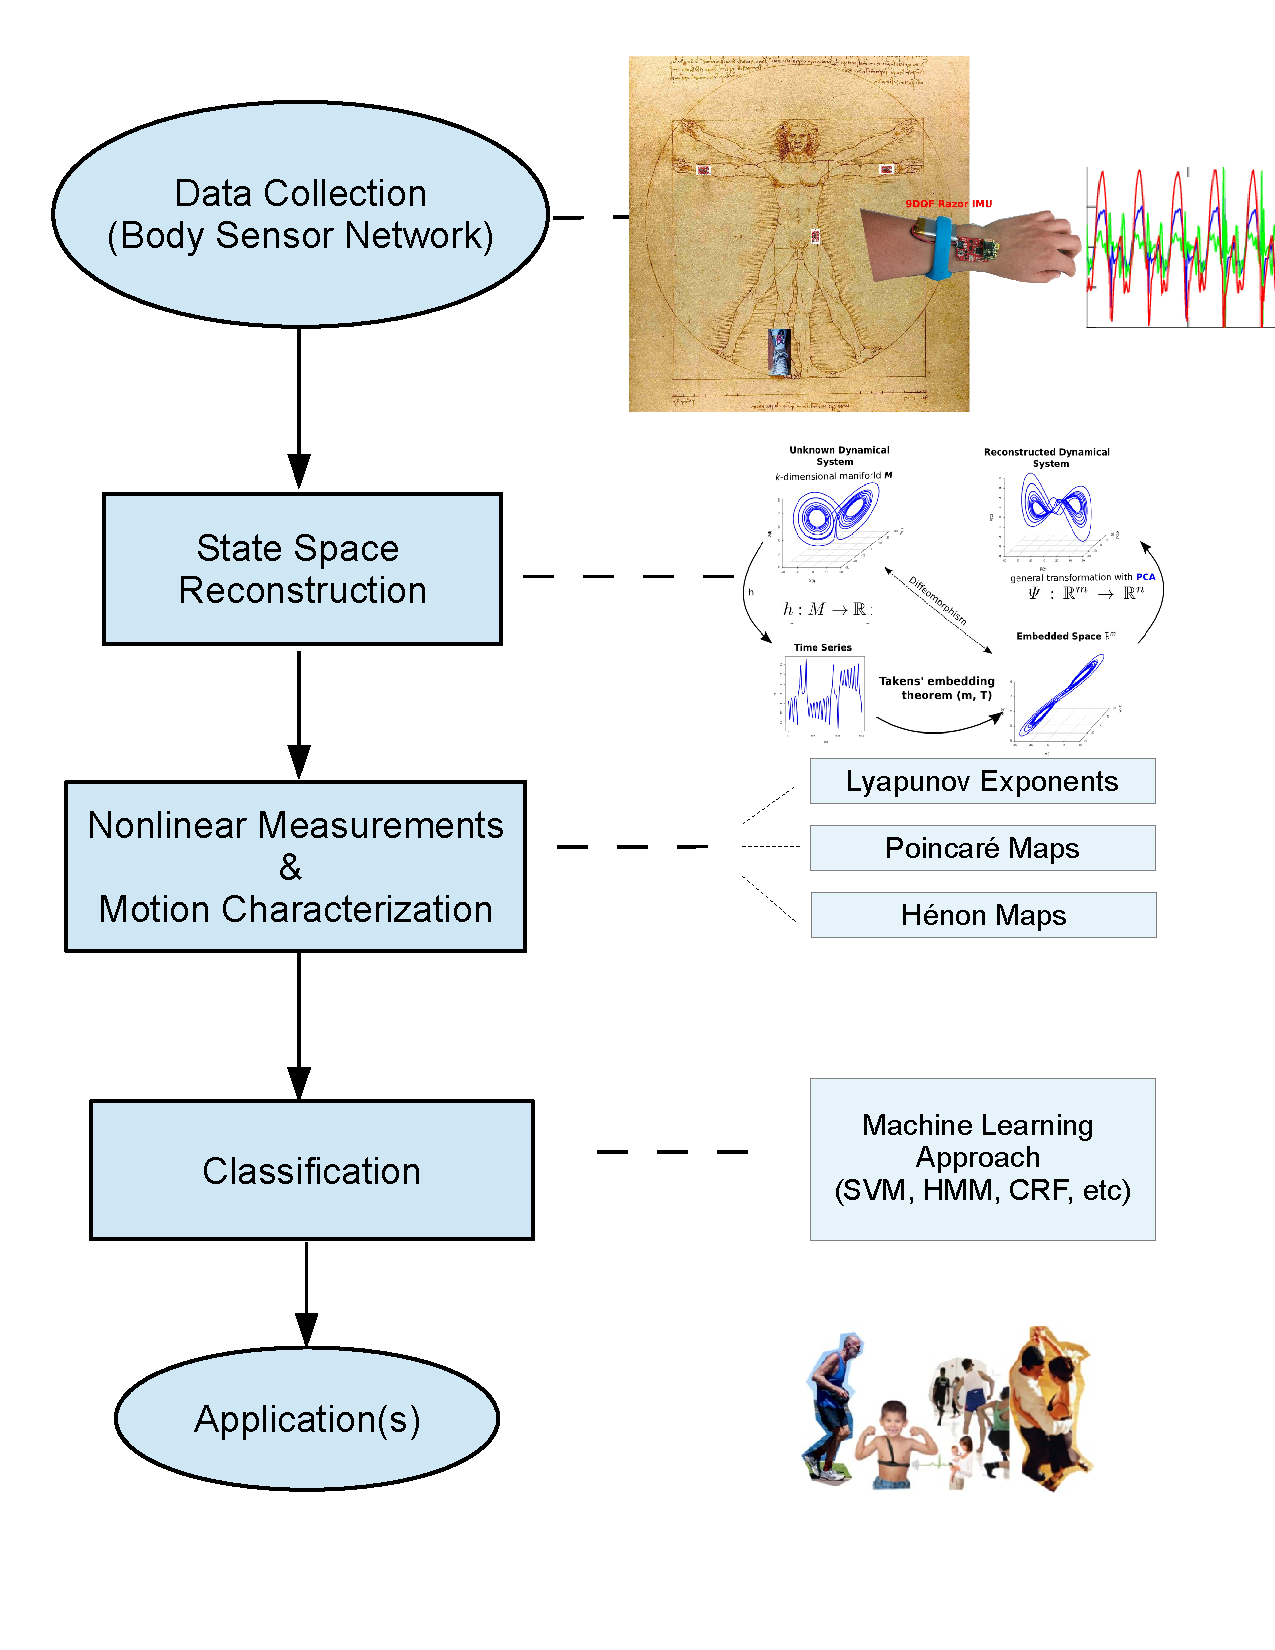
\includegraphics[width=0.9\textwidth]{proposedapproach_v1}
\caption[PA]{PhD Framework}
\label{fig:proposedapproach}
\end{figure}



Based on the proposed framework, 
tasks for the following 6 months are planned as follow:
\begin{itemize}[noitemsep,topsep=0pt,parsep=0pt,partopsep=0pt]
%  \item T1: 5 curses will be taken and they will be suggested by the doctoral committee.
\item T1 [February]: Review of state-of-the-art of machine learning methods 
for human activity recognition using wearable sensors.
\item T2 [March]: Define the human activity experiment and recruit subjects 
to collect data so as to test the proposed PhD framework by means of a suitable
machine learning algorithm.
\item T4 [April]: Write and submit a conferece paper in The 19th International Symposium
on Wearable Computers
\item T5 [May-June]: Update the hardware of the body sensor network by using
Bluetooth low energy devices and inductive wireless chargers. 
\item T6 [May-June]: Update the open source sofware library for the body sensor
network.
\item T6 [July]: Write the 9th month report and create a publication
plan for the next year.
% \item T3: Definition of the experiments and motion capture system.
% \item T4: Programming method to obtain the reconstructed attractor
% \item T5: Evaluate the nonlinear measurements and the motion characterization.


\item T9: Comparison of the proposed approach with recent methods.
\item T10 Writing, review and PhD thesis defence.
\end{itemize}

% Timeline is shown in the gantt chart 
% % (Figure \ref{fig:ganttchart})
% in which each year is divided into four periods (1 to 4).
% Additionally, it is an objective to write and publish at least two articles per year.
% 

% \begin{figure}[htbp!] 
% \begin{center}
%   \begin{gantt}{12}{12} %{rows}{columns}
%     \begin{ganttitle}
%       \numtitle{2014}{1}{2014}{1}
%       \numtitle{2015}{1}{2016}{4}
%       \numtitle{2017}{1}{2017}{3}
%     \end{ganttitle}
%     
%     \begin{ganttitle}
%       \numtitle{1}{1}{2}{1} % Titles with numbers
%       \numtitle{1}{1}{2}{1}
%       \numtitle{1}{1}{4}{1}
%       \numtitle{1}{1}{3}{1}
% %       \numtitle{1}{1}{3}{1}
%     \end{ganttitle}
%     
%   \ganttbar{T1}{0}{4}
%   \ganttbarcon{T2}{4}{2}
%   \ganttbarcon{T3}{5}{1}
%   \ganttbarcon{T4}{6}{2}
%   \ganttbarcon{T5}{6}{2}
%   \ganttbarcon{T6}{8}{1}
%   \ganttbarcon{T7}{8}{1}
%   \ganttbarcon{T8}{9}{1}
%   \ganttbarcon{T9}{9}{2}
%   \ganttbar{T10}{10}{2}
%   \end{gantt}
%   \caption[PA]{Gantt Chart for the research proposal}
% \label{fig:ganttchart}
%   \end{center}
% \end{figure}
  
  
  